%20 min preso!
\documentclass[xcolor=table,english,russian]{beamer}
\usepackage{beamerthemesplit}
\usepackage{wrapfig}
\usetheme{SPbGU}
\usepackage{pdfpages}
\usepackage{amsmath}
\usepackage{mathtools}
\usepackage{cmap}
\usepackage{subcaption}
\usepackage[utf8]{inputenc}
\usepackage[T1, T2A]{fontenc}
\usepackage[]{babel}
\usepackage{indentfirst}
\usepackage{amsmath}
\usepackage{tikz}
\usepackage{multirow}
\usepackage[noend]{algpseudocode}
\usepackage{algorithm}
\usepackage{algorithmicx}
\usepackage{fancyvrb}
\usetikzlibrary{calc}
\usetikzlibrary{shapes,arrows}
\usetikzlibrary{arrows,automata}
\usetikzlibrary{positioning}
\usetikzlibrary{fit}

\usepackage{kbordermatrix} % include package @ document preamble
\renewcommand{\kbldelim}{(} % change default array delimiters to parentheses
\renewcommand{\kbrdelim}{)}

\newcommand\mca{\multicolumn{1}{c}{\cellcolor{red}\textbf{\{a\}}}}
\newcommand\mcb{\multicolumn{1}{c}{\cellcolor{red}\textbf{\{b\}}}}

\usepackage{tabularx}
\newcolumntype{Y}{>{\raggedleft\arraybackslash}X}

\renewcommand{\thealgorithm}{}

\newtheorem{mytheorem}{Theorem}
\renewcommand{\thealgorithm}{}

\newcommand{\tikzmark}[1]{\tikz[overlay,remember picture] \node (#1) {};}
\def\Put(#1,#2)#3{\leavevmode\makebox(0,0){\put(#1,#2){#3}}}

\newcommand{\ltz}{$< 1$}


\tikzset{
    state/.style={
           rectangle,
           rounded corners,
           draw=black, very thick,
           minimum height=2em,
           inner sep=2pt,
           text centered,
           },
}

\beamertemplatenavigationsymbolsempty

\title[Kronecker Product CFPQ]{Поиск путей в графе с КС ограничениями через произведение Кронекера}
%\subtitle[YaccConstructor]{Parsing techniques for graph analysis}
% То, что в квадратных скобках, отображается в левом нижнем углу.
\institute[СПбГУ]{
JetBrains Research, Лаборатория языковых инструментов  \\
Санкт-Петербургский Государственный университет
}

% То, что в квадратных скобках, отображается в левом нижнем углу (прикольно).
\author[Егор Орачев, Илья Эпельбаум]{\textbf{Егор Орачев}, \textbf{Илья Эпельбаум} \\ Научный руководитель: Семен Григорьев}

\date{31 Августа 2020}


\begin{document}
{
\begin{frame}[fragile]
  \begin{table}
  \centering
  \begin{tabularx}{\linewidth}{YcX}
    
\includegraphics[height=1.5cm]{pictures/jetbrainsResearch.pdf} \hfill
    & \begin{minipage}[t]{0.3\textwidth}\center \vspace{-1cm}  JBR Interns 2020
      \end{minipage}
    & \hfill 
\includegraphics[height=1.5cm]{pictures/SPbGU_Logo.png}
  \end{tabularx}
  \end{table}
  \titlepage
\end{frame}
}

\begin{frame} \frametitle{Context-Free Path Querying}
  \begin{minipage}[m]{0.45\linewidth}
  \raisebox{-0.5\totalheight}{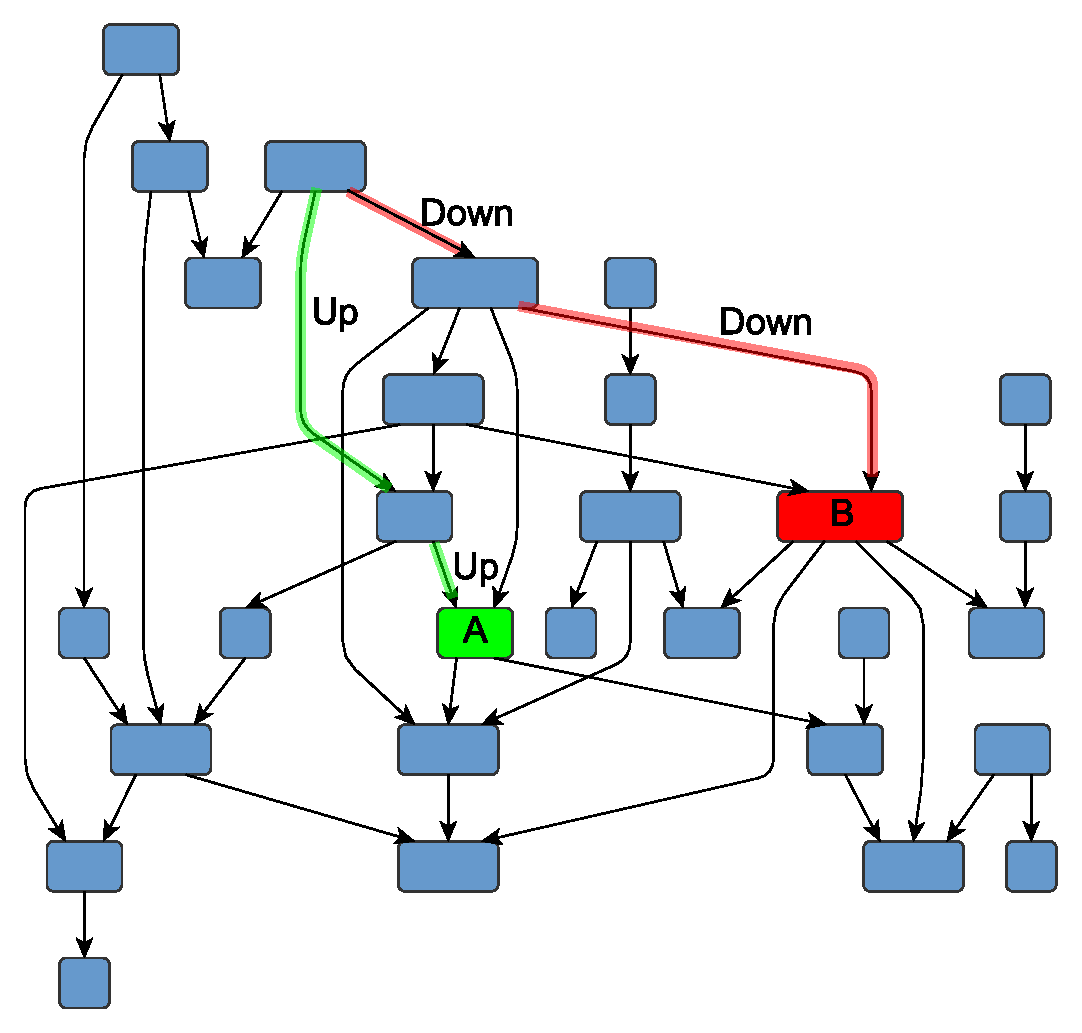
\includegraphics[width=\textwidth]{pictures/hierarchical.pdf}}
  \end{minipage}\hfill
  \begin{minipage}[m]{0.5\linewidth}
  Навигация в графе
  \begin{itemize}
        \item Находятся ли вершины A и B на одном уровне иерархии?
        \item Существует ли путь вида $\textbf{Up}^n \, \textbf{Down}^n$?
        \item Найти все такие пути $\textbf{Up}^n \, \textbf{Down}^n$, которые начинаются в вершине~А
  \end{itemize}
  \end{minipage}
\end{frame}

\begin{frame}[fragile] \frametitle{Семантика запросов}
    \begin{itemize}
        \item $\mathbb{G} = (\Sigma, N, P)$ --- контекстно-свободная грамматика
        \begin{itemize}
            \item $\Sigma$ конечное множество терминалов
            \item $N$ конечное множество нетерминалов
            \item $P$ конечное множество правил вывода
            \item $L(\mathbb{G},A) = \{ \omega \mid A \Rightarrow^* \omega \}, A \in N$
        \end{itemize}
        %\pause
        \item $G = (V,E,L)$ --- ориентированный граф с метками
        \begin{itemize}
            \item $v \xrightarrow{l} u \in E$
            \item $L \subseteq \Sigma$
        \end{itemize}
        %\pause
        %\item $p = v_0 \xrightarrow{l_0} v_1 \xrightarrow{l_1} \cdots \xrightarrow{l_{n-2}} v_{n-1} \xrightarrow{l_{n-1}} v_n$ --- path in $G$
        \item $\omega(\pi) = \omega(v_0 \xrightarrow{l_0} v_1 \xrightarrow{l_1} \cdots \xrightarrow{l_{n-2}} v_{n-1} \xrightarrow{l_{n-1}} v_n) = l_0 l_1 \cdots l_{n-1}$
        %\pause
        \item $R_A = \{ (n, m) \mid \exists n \pi m$, такой что $\omega(\pi) \in L(\mathbb{G},A)\}, A \in N$
    \end{itemize}
\end{frame}

\begin{frame}[fragile] \frametitle{Существующие решения}
    \begin{itemize}
        \item Решения, основанные на различных техниках парсинга \\ (CYK, LL, LR, etc.)
        %\pause
        \item Решения, основанные на матричных операция
        %\pause
        \item Существующие решения слишком \textit{тяжеловесны} для запросов, выраженных регулярными ограничениями\footnote{Reqular path quering (RPQ) --- поиск путей с регулярными ограничениями}
        \item Все существующие решения работают только с КС грамматикой в нормальной форме (Нормальная форма Хомского)
        %\pause
        \item \textbf{Трансформация требует дополнительного времени на обработку и приводит к разрастанию грамматики }
    \end{itemize}
\end{frame}

\begin{frame}[fragile] \frametitle{Мотивация разработки нового алгоритма}
    \begin{itemize}
        \item Работает с достаточно \textit{хорошим} представлением входной грамматики, которое не требует дополнительной трансформации в нормальную форму и не приводит к увеличению числа продукций
        \item Реализуется в терминах операций линейной алгебры
        \item Приемлем для запросов, выраженных регулярными ограничениями
        \item Позволяет получать информацию не только о достижимости вершин, но и о путях, соединяющих эти вершины
    \end{itemize}
\end{frame}

\begin{frame}[fragile] \frametitle{Задачи Егора}
    \begin{itemize}
        \item Формализация алгоритма, описание \textit{наивной} реализации в категории операций линейной алгебры с использованием булевой матричной декомпозиции
        \item Оформление текста статьи для конференции \textbf{2020 ACM SIGMOD}
        \item Подготовка \textbf{LUBM} датасета для тестирования регулярных запросов
    \end{itemize}
\end{frame}

\begin{frame}[fragile] \frametitle{Задачи Ильи}
    \begin{itemize}
        \item Реализация \textit{наивной} версии алгоритма на основе библиотеки \textbf{PyGraphBLAS}\footnote{PyGraphBLAS --- python-обертка для SuiteSparse C --- реализации GraphBLAS API для работы с графами в терминах операций линейной алгебры}
        \item Реализация на основе \textbf{PyGraphBLAS} извлечения путей из \textit{индекса}, построенного в ходе выполнения основного алгоритма
        \item Проведение CFPQ и RPQ замеров работы алгоритма построения индекса и алгоритма извлечения путей
    \end{itemize}
\end{frame}

\begin{frame}[fragile] \frametitle{Заключение}
    \begin{itemize}
        \item Выполнены задачи по разработке и реализации алгоритма
        \item Получены \textit{оптимистичные} и воодушевляющие результаты работы алгоритма относительно \textit{классического} матричного аналога
        \item Подготовлена статья для конференции \textbf{2020 ACM SIGMOD} 
    \end{itemize}
\end{frame}

\begin{frame}[fragile] \frametitle{Дальнейшие задачи}
  \begin{itemize}
    \item Исследование проблемы извлечения всех путей
    \item Детальное сравнение с классическим матричным алгоритмом
    \item Реализация алгоритма на GPGPU с использованием разреженных булевых матриц
    \item Модификация алгоритма для распределенного вычисления 
    \item Интеграция алгоритма с графовой базой данных (RedisGraph)
\end{itemize}
\end{frame}

\begin{frame} \frametitle{Контакты}
    \begin{itemize}
        \item Семен Григорьев:
        \begin{itemize}
          \item \href{mailto:s.v.grigoriev@spbu.ru}{s.v.grigoriev@spbu.ru}
          \item \href{mailto:Semen.Grigorev@jetbrains.com}{Semen.Grigorev@jetbrains.com}
        \end{itemize}
        \item Рустам Азимов:
        \begin{itemize}
            \item \href{mailto:rustam.azimov19021995@gmail.com}{rustam.azimov19021995@gmail.com}
            \item \href{mailto:Rustam.Azimov@jetbrains.com}{Rustam.Azimov@jetbrains.com}
        \end{itemize}
        \item Екатерина Шеметова:  \href{mailto:katyacyfra@gmail.com}{katyacyfra@gmail.com}
        \item Егор Орачев: \href{mailto:egor.orachev@gmail.com}{egor.orachev@gmail.com}
        \item Илья Эпельбаум: \href{mailto:iliyepelbaun@gmail.com}{iliyepelbaun@gmail.com}
        \vspace{0.5cm}
        \item Датасет: \href{https://github.com/JetBrains-Research/CFPQ_Data}{https://github.com/JetBrains-Research/CFPQ\_Data}
        \item Реализация: \href{https://github.com/YaccConstructor/RedisGraph}{https://github.com/YaccConstructor/RedisGraph}
    \end{itemize}
    \vspace{0.1cm}
\end{frame}

\end{document}